\documentclass[a4paper,12pt]{article}

\usepackage{estilos}

\pagestyle{empty}

\begin{document}
\begin{center}%
  \begin{figure}[H]%
    \hspace*{-.5in}{\begin{minipage}[H]{.05\columnwidth}%
      \centering
      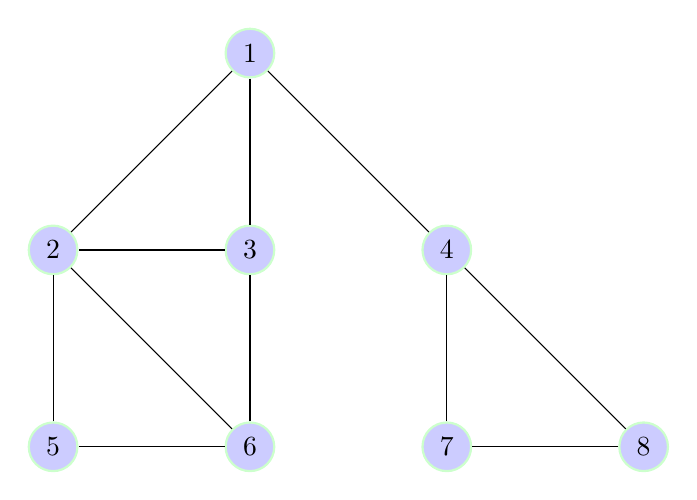
\begin{tikzpicture}{node distance=1.3cm,>=stealth',bend angle=45, auto}
        {

          \tikzstyle{place}=[circle,thick,draw=green!20,fill=blue!20,minimum size=6mm]
          \tikzstyle{texto}=[]
          \begin{scope}

            \node [place] (c1) {$2$};

            \node [place] (c2) [right of=c1,xshift=1.5cm] {$3$}
            edge [] (c1);

            \node [place] (c3) [above of=c2,yshift=1.5cm] {$1$}
            edge [] (c1)
            edge [] (c2);

            \node [place] (c4) [below of=c2,yshift=-1.5cm] {$6$}
            edge [] (c2)
            edge [] (c1);

            \node [place] (c5) [below of=c1,yshift=-1.5cm] {$5$}
            edge [] (c1)
            edge [] (c4);

            \node [place] (c6) [right of=c2,xshift=1.5cm] {$4$}
            edge [] (c3);

            \node [place] (c7) [below of=c6,yshift=-1.5cm] {$7$}
            edge [] (c6);

            \node [place] (c8) [right of=c7,xshift=1.5cm] {$8$}
            edge [] (c7)
            edge [] (c6);


          \end{scope}
        }
        \end{tikzpicture}
      \end{minipage}}
      \begin{center}
      \vspace{-2.5in}{\begin{minipage}{.05\columnwidth}%
        \centering%
        \begin{tikzpicture}{node distance=1.3cm,>=stealth',bend angle=45, auto}
          {

            \tikzstyle{place}=[circle,thick,draw=green!20,fill=blue!20,minimum size=6mm]
            \tikzstyle{texto}=[]
            \begin{scope}

              \node [place] (c1) [label=left:\textcolor{black}{$2$},label=right:\textcolor{black}{$1$}]{$2$};

              \node [texto] (c2) [right of=c1,xshift=1.5cm] {};

              \node [place] (c3) [above of=c2,yshift=1.5cm,label=right:\textcolor{black}{$1$},label=left:\textcolor{black}{$1$}] {$1$}
              edge [post] (c1);

              \node [place] (c4) [below of=c1,yshift=-.5cm,label=right:\textcolor{black}{$1$},label=left:\textcolor{black}{$3$}] {$3$}
              edge [pre] (c1)
              edge [bend right,dashed] (c3) ;

              \node [place] (c5) [below of=c4,yshift=-.5cm,label=right:\textcolor{black}{$2$},label=left:\textcolor{black}{$4$}] {$6$}
              edge [pre] (c4)
              edge [bend left=60,dashed] (c1) ;

              \node [place] (c6) [right of=c2,xshift=1.5cm,label=right:\textcolor{black}{$6$},label=left:\textcolor{black}{$6$}] {$4$}
              edge [pre] (c3);

              \node [place] (c7) [below of=c6,yshift=-.5cm,label=right:\textcolor{black}{$6$},label=left:\textcolor{black}{$7$}] {$7$}
              edge [pre] (c6);

              \node [place] (c8) [below of=c5,yshift=-.5cm,label=right:\textcolor{black}{$2$},label=left:\textcolor{black}{$5$}] {$5$}
              edge [pre] (c5)
              edge [bend left=65,dashed] (c1) ;

              \node [place] (c9) [below of=c7,yshift=-.5cm,label=right:\textcolor{black}{$6$},label=left:\textcolor{black}{$8$}] {$8$}
              edge [pre] (c7)
              edge [bend right=60,dashed] (c6) ;
            \end{scope}
          }
        \end{tikzpicture}
      \end{minipage}}
    \end{center}
  \end{figure}%
\end{center}%
\begin{figure}[H]
\caption{Un grafo no dirigido y su árbol de recorrido en profundidad.}
\end{figure}
\end{document}
